\documentclass[10pt,letterpaper]{article}
\usepackage[margin=0.87in]{geometry}
\usepackage[T1]{fontenc}
\usepackage[utf8]{inputenc}
\usepackage{lmodern}
\usepackage{microtype}
\usepackage{amsmath,amssymb,amsthm,mathtools,mathrsfs}
\usepackage{booktabs,array,tabularx,longtable}
\usepackage{enumitem}
\usepackage{xcolor}
\usepackage{hyperref}
\usepackage{fancyhdr}
\usepackage{tikz}
\usetikzlibrary{arrows.meta,positioning,calc}
\usepackage{titlesec}
\definecolor{navy}{RGB}{24,46,79}
\definecolor{teal}{RGB}{8,91,106}
\hypersetup{colorlinks=true,linkcolor=navy,urlcolor=teal,citecolor=navy,pdftitle={Formalized Awareness of AMLD Federations and Board-Players v0.3},pdfauthor={Research draft prepared for Brian Tenneson}}
\titleformat{\section}{\Large\bfseries\color{navy}}{\thesection}{0.7em}{}
\titleformat{\subsection}{\normalsize\bfseries\color{teal}}{\thesubsection}{0.7em}{}
\pagestyle{fancy}\fancyhf{}\fancyhead[L]{\small\textcolor{navy}{AMLD Federation Awareness --- ATLAS repaired and re-audited}}\fancyhead[R]{\small v0.3}\fancyfoot[C]{\thepage}\setlength{\headheight}{15pt}
\setlist[itemize]{leftmargin=*,itemsep=2pt,topsep=3pt}
\setlist[enumerate]{leftmargin=*,itemsep=2pt,topsep=3pt}
\newtheorem{definition}{Definition}[section]
\newtheorem{theorem}[definition]{Theorem}
\newtheorem{proposition}[definition]{Proposition}
\newtheorem{lemma}[definition]{Lemma}
\newtheorem{corollary}[definition]{Corollary}
\newtheorem{conjecture}[definition]{Conjecture}
\theoremstyle{remark}\newtheorem{remark}[definition]{Remark}
\newtheorem{question}[definition]{Research question}
\newcommand{\AMLD}{\mathsf{AMLD}}
\newcommand{\ATP}{\mathsf{ATP}}
\newcommand{\SIC}{\mathsf{SIC}}
\newcommand{\GBG}{\mathsf{GBG}}
\newcommand{\F}{\mathcal{F}}
\newcommand{\Ag}{\mathcal{A}}
\newcommand{\KB}{K_0}
\newcommand{\Cn}{\operatorname{Cn}}
\newcommand{\Prf}{\operatorname{Pr}}
\newcommand{\View}{\operatorname{View}}
\newcommand{\Wit}{\operatorname{Wit}}
\newcommand{\Self}{\operatorname{Self}}
\newcommand{\Tag}{\operatorname{Tag}}
\newcommand{\Out}{\operatorname{Out}}
\newcommand{\Leg}{\operatorname{Legal}}
\newcommand{\Act}{\operatorname{Act}}
\newcommand{\Tr}{\operatorname{Trace}}
\newcommand{\E}{\mathcal{E}}
\newcommand{\N}{\mathbb{N}}
\newcommand{\Norm}{\operatorname{Norm}}
\begin{document}
\begin{center}
{\LARGE\bfseries\color{navy} Formalized Awareness of AMLD Federations\\[3pt] and Board-Players}\\[9pt]
{\large A sibling theory to \emph{Formalized Self-Awareness and Self-Aware Structures}}\\[8pt]
{\normalsize Tagged settlement profiles, GBG/GBG$^+$, Player Zero, three $B^*$ controllers,\\ verifier-grounded reflection, Gestalt surplus, and countably fair clocks}\\[10pt]
\textbf{ATLAS additional repairs and re-audit --- working draft v0.3 --- 25 October 2026}\\[3pt]
Prepared as a research-development draft for \textbf{Brian Tenneson}\\[3pt]
\textit{Not author-approved, published, or mechanically verified; including additional ATLAS re-audit repairs}
\end{center}
\vspace{0.35em}
\noindent\colorbox{navy!7}{\parbox{0.965\linewidth}{\small\textbf{Scope and audit status.} This manuscript is a sibling, not an alteration of the original self-awareness article. Version 0.3 retains the nine v0.1 repairs and addresses additional defects identified in the independent v0.2 re-audit. Mathematical proofs below are conditional where stated; no proof kernel has mechanically checked this manuscript. It reports no new eight-ATP AMLD execution, awareness certificate, settlement, or performance result. \emph{Awareness} remains a formal warrant/self-description notion, not a claim of phenomenal consciousness.}}
\begin{abstract}
The passage from a semi-ideal computer (SIC) to an automated theorem prover (ATP), and then to an automated metalogical decider (AMLD), is not a lexical substitution. A SIC has a monotone stage-output map; an AMLD has role-differentiated candidate production, verifier-gated object and meta-records, clocked service, possibly nonmonotone Board/GBG state, and charged resource consumption. We define tagged, clocked AMLD federation profiles, with separately pinned object/meta-verification interfaces, and two levels of formal awareness: syntactic provability self-description and accessible, independently witnessed epistemic reflection. For a proposed federation containing five specialist ATPs $P,R,D,I,C$ and three controller ATPs $B_0^*,B_1^*,B_2^*$, we define a single composite legal-transition game rather than asserting an unproved equivalence of three GBG$^+$ components. We distinguish local awareness, federation awareness, mutual awareness, and coalition-dependent reflective surplus. We give rigorous countermodels to the automatic elevation of individual awareness into collective awareness and to free reflective ascent. A finite Horn construction witnesses genuine three-source dependency relative to frozen local information. We also prove that a countably infinite federation admits a computable, surjective, \emph{recurrently fair} one-service-per-tick clock; a bijective clock alone does not suffice. The construction $\chi(t)=a_{v_2(t+1)}$ serves agent $a_i$ at exact intervals of $2^{i+1}$ ticks. We distinguish this mathematical existence result from infinite simultaneous deployment or infinite service under a finite charged budget. The result is a proposed technical foundation for the study of awareness and reflective surplus in AMLD-class federations.
\end{abstract}
\tableofcontents
\newpage
\section{The promotion question is a problem in definitions}
The source manuscript \emph{Formalized Self-Awareness and Self-Aware Structures} [1] moves from SICs to tagged ATP profiles and a primitive provability predicate. A proposal to ``promote'' SIC to ATP and ATP to AMLD is mathematically fruitful, but a literal substitution is false in general: not every SIC is an effective ATP, and not every ATP is an AMLD with a five-role settlement interface. More seriously, the source SIC state-map is cumulative, whereas a board position or controller queue may change nonmonotonically.

We therefore seek a sequence of \emph{faithful representations}, rather than a replacement of words. The intended architecture is
\[
\boxed{\text{SIC theory}\ \longrightarrow\ \text{tagged ATP theory}\ \longrightarrow\ \text{AMLD federation theory}}
\]
with each arrow conditional on the appropriate typing, soundness, and trace-interpretation hypotheses. Nothing requires all axioms or all theorems on the left to transfer to every object on the right.

\subsection{Three levels of interpretation}
\begin{description}[style=nextline,leftmargin=0pt]
\item[Level S: SIC.] An abstract stage process $M=(C,H)$ over a formula domain $Y$, with $C(\Gamma,1)=\Gamma$, $C(\Gamma,n)\subseteq C(\Gamma,n+1)$, persistent halting, and stabilization after halting [1].
\item[Level A: ATP.] A SIC intended to enumerate formal consequences or search for a target, with sound/checkable proof behavior separately established. A role label is not sufficient evidence of genuine prover behavior.
\item[Level F: AMLD.] A typed federation with designated settlement roles, one or more lawful board-player controllers, verifier gates, persistent certified record, resource accounting, and a global service clock. It may be represented by an SIC recording cumulative histories, but its changing instantaneous Board state is not itself a SIC cumulative output.
\end{description}

\begin{proposition}[Naive state promotion fails]
The evolving complete Board state of a legal GBG/AMLD process need not satisfy the SIC monotonicity axiom $C(\Gamma,n)\subseteq C(\Gamma,n+1)$.
\end{proposition}
\begin{proof}
Consider a legal board move exchanging a location's occupant token from $p$ to the empty token $E$. The stage-$n$ state contains the proposition ``this location is occupied by $p$,'' but the successor state does not. Regard complete current states as sets of such atomic observations. Then neither stage inclusion nor persistence of those observations is assured. This does not contradict SIC theory, because the current Board state has a different type from a cumulative formula-output history.
\end{proof}

\begin{proposition}[Total cumulative-history SIC encoding]
Let $S$ be an effectively coded set of finite configurations and let $\delta:S\to S$ be a total computable successor (with any declared terminal configurations fixed). On the effective record domain $Y=S\times\N$ define the total unary record successor
\[
T(s,j)=(\delta(s),j+1).
\]
For \emph{every} subset $\Gamma\subseteq Y$, including infinite subsets, and every $m\ge1$, define
\[
C(\Gamma,m)=\{T^k(x):x\in\Gamma,\ 0\le k<m\},\qquad H(\Gamma,m)=0.
\]
Then $(C,H)$ satisfies the full SIC axioms, whose domain is $\mathcal P(Y)\times\N^+$. Its restriction to \emph{finite} inputs is finite-stage-coded and computationally effective. From $\Gamma_0=\{(s_0,0)\}$ it records the first $m$ time-indexed configurations of the deterministic run.
\end{proposition}
\begin{proof}
The functions are defined set-theoretically for \emph{every} $\Gamma\subseteq Y$ and every positive stage. By construction $C(\Gamma,1)=\Gamma$ and $C(\Gamma,m)\subseteq C(\Gamma,m+1)$, even for infinite inputs. The constant-zero halting map satisfies persistent halting and post-halting stability vacuously. For a finite input $\Gamma$, the stage output is finite and can be computed by iterating the total effective map $T$ at most $m-1$ times per input record. No algorithm for coding an arbitrary infinite output set is claimed. For the singleton seed, induction gives $T^k(s_0,0)=(\delta^k(s_0),k)$, establishing the trace-prefix claim. This construction deliberately makes no claim that the SIC recognizes terminal settlement.
\end{proof}
\begin{remark}[Scope of the embedding]
The second coordinate distinguishes repeated terminal states at different times. These records are \emph{execution-history data}, not automatically object-level certified theorems. To record a nondeterministic or distributed run, first freeze a computable resolution of scheduler/seed/choices into the effective successor and retain the actual event log; the theorem does not construct a computable resolver for arbitrary infinite nondeterminism. A separate halting SIC is possible only after defining a persistent terminal policy on \emph{all} permitted inputs.
\end{remark}

\section{A tagged AMLD federation profile}
\begin{definition}[Federation profile]
An AMLD federation profile is a typed record
\[
\begin{aligned}
\mathfrak P=(&\Ag,\rho,\mathbf G,\mathbf B,\chi,F,\Gamma,T,V_{\rm obj},V_{\rm meta},K_0,\\
&\mathsf{Auth},\mathsf{Cost},\mathcal L,\mathcal E,\mathsf{View},\mathsf{Witness},\mathsf{Reflect},\\
&\mathsf{Snapshot},\mathsf{Exit},\mathsf{Ext},\mathsf{Tag}).
\end{aligned}
\]
Here $\Ag$ is an effectively indexed agent set; $\rho$ assigns actual authorized capabilities; $\mathbf G,\mathbf B$ encode a rule-complete game and mutable control state; $\chi$ is the global service-owner clock; $F,\Gamma,T$ are the frozen object calculus, hypotheses, and target; $V_{\rm obj}$ and $V_{\rm meta}$ are pinned independently invoked, \emph{typed} checker interfaces; $K_0$ is the immutable initial record union specified below; $\mathsf{Auth}$ governs access and actions, $\mathsf{Cost}$ all charged work, and $\mathcal L$ the durable event/receipt ledger. The frozen meta-domain $\mathcal E$, authorized views $\mathsf{View}$, accepted-witness relation $\mathsf{Witness}$, receipt constructor $\mathsf{Reflect}$, and historical snapshot authentication $\mathsf{Snapshot}$ have the contracts specified below. The remaining fields fix legal exit, optional modules, and the actual denotations of agent/federation tags.
\end{definition}

The mandatory five settlement specialties are $P$ (proof), $R$ (refutation), $D$ (dependence), $I$ (independence), and $C$ (contradiction). In the proposed \emph{eight-ATP core} we take
\[
\Ag_8=\{P,R,D,I,C,B^*_0,B^*_1,B^*_2\}.
\]
Each symbol is a \emph{proposed} independently functioning ATP with a correctly interpreted tag and an individually certified self-model; these requirements are hypotheses, not facts established for an existing installation. A separate checker is not a ninth voting ATP. Multiple ATPs may carry the same specialty, and cardinality need not be eight. The earlier three-$B^*$ attestation and primes adaptation show process-distinct controllers and bounded finite checking, \emph{not} eight autonomous ATP implementations, eight reflective certificates, or complete AMLD settlement [9].

\begin{definition}[Frozen three-multiarticle \emph{record} BANK]
Let $M_1,M_2,M_3$ each be sets of records containing at least source identifier, native calculus, source hypotheses, conclusion, proof/certificate identifier, native-verifier receipt, and provenance. Preserve the source identifier \emph{inside each record} so equality cannot conflate two distinct source judgments. The intended starting ledger is their ordinary set union,
\[
\boxed{K_0=M_1\cup M_2\cup M_3.}
\]
This is an immutable \emph{record union}, not automatically a jointly admissible or consistent object-language axiom set. Let $\mathsf{Adm}_{F,\Gamma,V_{\rm obj}}(K_0)$ denote precisely the entries whose judgments can be translated to the fixed target calculus $F$ and admitted under the fixed hypothesis context $\Gamma$ by $V_{\rm obj}$, with accepted translation/checker receipts. All other source-certified records remain readable with native scope, but are \emph{not} unconditionally imported as $F$-theorems. A source proof under $\Gamma_i$ cannot discharge $\Gamma_i\setminus\Gamma$ by renaming or union. In the composite state below, $k$ is the \emph{accepted object-judgment store}, initialized as $k_0=\mathsf{Adm}_{F,\Gamma,V_{\rm obj}}(K_0)$; the full source archive $K_0$ remains a separately typed immutable resource. This keeps unimported native records out of the current-calculus theorem BANK.
\end{definition}

No recursive consequence mining is performed during initialization. Unchecked prompt histories and candidate conjectures belong in a separate untrusted archive. The union is \emph{not} the binary multiarticle zip operation $m$, deletes no source entry, and is distinct from the three controller identities $B^*_0,B^*_1,B^*_2$.

\begin{definition}[Frozen certificate and view interfaces]
The object checker $V_{\rm obj}$ accepts only exact judgments $(F,\Gamma,\varphi,\pi,\text{profile digest})$ with complete undischarged-premise metadata. The meta-checker $V_{\rm meta}$ accepts typed judgments concerning a tagged agent/federation, named epoch and authorized evidence, including authentic hashes of receipts and view snapshots. For each epoch $t$, the policy $\mathsf{View}_{i}(t)$ selects only accepted records actually accessible to subject $i$ at $t$; $\mathsf{Snapshot}$ binds claims about past access to preserved signed or replay-checkable historical views. The predicate $\mathsf{Witness}(r,\varphi,i,t)$ requires a positive correctly scoped $V_{\rm meta}$ receipt. This is \emph{acceptance relative to a pinned checker}; its semantic soundness, $\mathsf{Witness}(r,\varphi,i,t)\Rightarrow\varphi$, is a separately named assumption (SND), not a consequence of possessing a receipt. The partial constructor $\mathsf{Reflect}$ may turn a valid historical witness and authenticated snapshot into a \emph{new candidate} reflective receipt, which must itself pass $V_{\rm meta}$. None of these interfaces is defined by self-report alone.
\end{definition}

\subsection{Certification is not consensus}
A role or controller may propose a statement, but accepted object theoremhood requires $V_{\rm obj}$ and accepted meta-warrant requires $V_{\rm meta}$. They may share executable code but retain different typed judgments. Neither a peer vote nor an object-level proof alone certifies who had accessible knowledge at a past epoch. Admitted knowledge, raw logs, and current access rights remain distinct [3--5].

\section{Generalized board games and the three board-players}
The underlying GBG uses a location report
\[
\ell\in[A\to(P_{\mathrm{tok}}\cup\{E\})],
\]
where $A$ is the set of board locations, $P_{\mathrm{tok}}$ the occupant tokens, and $E$ the \emph{empty token}, not the empty set. The complete legal state may be $s=(\ell,\tau,\eta)$, where $\tau$ records service/turn information and $\eta$ includes any other legally relevant state. A changed report alone does not establish that any legal motion occurred: a tagged rule and state-to-state proof are required [6].

The original GBG$^+$ proposal [7] distinguishes the board-state coordinate $B$ from the unique special player $P_0=B^*$. It grants $B^*$ no extra-system powers: the board-player acts only by legal enlarged-game transitions. The proposal also treats certified memory, reflection and scheduling as optional properties, not automatic consequences of merely adding the board-player.

\begin{definition}[Eight-agent three-controller composite game]
This paper defines a \emph{new composite game}, not an ordinary GBG$^+$ with three copies of its unique $P_0$. Fix the five distinct specialist identities $S_5=\{P,R,D,I,C\}$ and three controller identities $Q_3=\{B_0^*,B_1^*,B_2^*\}$. Take the disjoint agent union $\Ag_8=S_5\sqcup Q_3$. A complete composite state is
\[
s=(g,b_0,b_1,b_2,q,k,\lambda,c,t,z),
\]
where $g$ is a rule-complete ordinary GBG state containing the specialist-local and shared rule-relevant coordinates; $b_j$ is controller $j$'s state; $q$ contains typed handoff queues; $\lambda$ is an append-only event/receipt ledger; $c$ is accrued cost; $t$ is global service index; and $z$ is status. Freeze a single clock $\chi:\N\to\Ag_8$. For each owner $i$ and action label $a$, specify a \emph{partial, deterministic} rule
\[
r_{i,a}:D_{i,a}\longrightarrow\mathsf S_8,\qquad D_{i,a}\subseteq\mathsf S_8,
\]
whose guard checks $\chi(t)=i$, the owner's exact permissions, the underlying GBG legality when $g$ changes, verifier gates for certified commits (the $k$ coordinate changes only on accepted $V_{\rm obj}$ judgments), and accounting. Every legal step increments $t$, records actor/action/state delta, and charges declared work. A scheduler-owned no-op is permitted only when explicitly enabled and logged. No $B_j^*$ may mutate a protected coordinate through an undeclared shortcut. The resulting tagged partial-rule graph is the \emph{three-controller extension} $G^{\langle3B\rangle}$.
\end{definition}

\begin{proposition}[Well-defined tagged game and conditional passive projection]
If the state codes, guards, and each action's successor are well-formed/effective, the tagged rules above define a rule-complete enlarged GBG. For the \emph{passive subclass} in which every $B_j^*$ action changes only administrative state, ordinary-player action guards/successors are unchanged on the projected $g$-coordinates, and no infinite controller-only tail prevents an ordinary move, forgetting board-only coordinates and finite administrative stuttering projects every composite history onto a legal underlying $G$ history (not necessarily every possible $G$ history). This statement concerns the \emph{legality of projected histories}, not surjectivity onto all underlying histories or a global equivalence of games.
\end{proposition}
\begin{proof}
By definition, a complete state determines the owner, the set of enabled tagged rules, and the unique successor for each enabled rule, hence rule completeness. In the passive subclass, deleting a controller step does not alter $g$ or any subsequent ordinary action's legality. Induction on the number of retained ordinary moves shows that the projected sequence obeys the original tagged partial rules. The no-infinite-stutter condition prevents an endless administrative tail from masquerading as a maximal ordinary play. No such projection is claimed for active control.
\end{proof}

\begin{remark}[Relation to three GBG$^+$ components]
Each source GBG$^+$ has exactly one distinguished $P_0=B^*$. Three separate components can be \emph{amalgamated} into $G^{\langle3B\rangle}$ only after identifying their common five specialist identities and supplying a consistency map for shared $g$, a synchronized owner clock, cross-component queues, and step-by-step preservation of guards/successors. A naive Cartesian product would duplicate the specialists and permits incompatible independent clocks. No unconditional product--composite equivalence is claimed here. Three $B^*$s are \emph{three distinct controller agents}, never the mutable board-state coordinates $b_j$.
\end{remark}

\begin{proposition}[Legal projection requires a hypothesis]
Erasing an actively scheduling or board-mutating controller from an enlarged composite GBG need not leave a legal history of the original GBG. Projection-conservativity is valid for an appropriate passive, stutter-safe subclass, but not guaranteed by the presence of board-players alone.
\end{proposition}
\begin{proof}
The controller might select which ordinary role moves next or alter a legal-state coordinate. Removing that step can change the enabled-action sequence. By contrast, if every controller step is a passive administrative stutter leaving all ordinary coordinates and legal successors unchanged, and no infinite stutter postpones ordinary progress, deleting finitely many such steps preserves ordinary legal histories. This is the same distinction established for the passive GBG$^+$ extension in [7].
\end{proof}

\section{Two self-awareness ladders: proof and knowledge}
\begin{definition}[Names and provability syntax]
Fix a closed tag $t_{\F}=\langle\F\rangle$ for the complete frozen federation profile and an injective formula-naming map $Q$. The syntactic self-description ladder is
\[
\theta_0^{\F}=\AMLD(t_{\F}),\qquad
\theta_{n+1}^{\F}=\Prf_{\F}(t_{\F},Q(\theta_n^{\F})).
\]
Here $\Prf_{\F}$ must receive an exact declared meaning: e.g., the federation outputs an independently checked proof of the named formula in its frozen profile. Syntax alone does not ensure that its asserted proofs occurred.
\end{definition}

\begin{definition}[Verifier-grounded collective knowledge]
Let $\E_{\F}$ be a declared domain of admissible federation-level meta-propositions; let $\View_{\F}(t)$ be its \emph{currently authorized and accessible} record view; and let $\Wit_V(r,\varphi)$ express that $r$ is an independently accepted and correctly scoped witness for $\varphi$, with correct type, subject, verifier identity, and provenance. Soundness of such acceptance is a distinct assumption (SND). Put
\[
\boxed{K_{\F,t}\varphi\quad\Longleftrightarrow\quad
\varphi\in\E_{\F}\ \wedge\ \exists r\in\View_{\F}(t)\;\Wit_V(r,\varphi).}
\]
Define $K_{i,t}\varphi$ similarly using agent $i$'s epistemic domain and authorized view; local and collective accessibility need not coincide.
\end{definition}

\begin{proposition}[Factivity requires checker soundness]
If (SND) holds for all meta-witnesses in the federation's authorized view at epoch $t$, then $K_{\F,t}\varphi\Rightarrow\varphi$ for every admitted $\varphi$. Without (SND), positive checker acceptance alone does not establish this semantic implication.
\end{proposition}
\begin{proof}
By the definition of $K_{\F,t}$, obtain an accessible accepted witness $r$ for $\varphi$. Apply (SND) to conclude $\varphi$. To see why (SND) matters, take a checker that accepts an incorrect but properly scoped record for a false proposition; the knowledge predicate, understood as verifier-grounded acceptance, holds while the proposition is false. This illustrates a failure of checker soundness, not a permissible claim of sound certified knowledge.
\end{proof}

The $\theta$-ladder is a ladder of \emph{named proof-output assertions}; the $K$-ladder is one of \emph{certified accessible warrants}. They are separate until proof-output events have the exact metadata required by the pinned $V_{\rm meta}$, $\mathsf{Witness}$, $\mathsf{View}$ and $\mathsf{Snapshot}$ interfaces [1,2,4]. In particular, a claim $K_{\F,t}\varphi$ about a past epoch requires authentication of \emph{that historical view}, not merely today's receipt for $\varphi$. The statement $\AMLD(t_{\F})$ itself refers to the exact frozen profile: reorganization may require a newly tagged epoch.

\begin{theorem}[No automatic federation awareness]
For $\Ag_8$, the conjunction of all eight warranted personal self-identifications does not, under the preceding definitions alone, imply warranted federation self-identification:
\[
\bigwedge_{i\in\Ag_8}K_{i,t}\ATP(\langle i\rangle)\ \not\models\ K_{\F,t}\AMLD(\langle\F\rangle).
\]
\end{theorem}
\begin{proof}
Provide each $i$ an accepted accessible witness for $\ATP(\langle i\rangle)$ and admit that formula to $\E_i$. Let the federation have no accessible accepted witness for $\AMLD(\langle\F\rangle)$, or omit that proposition from $\E_{\F}$. Every conjunct on the left holds, while the right is false by definition. Thus local self-awareness and correct collective organization are insufficient without a collective warrant.
\end{proof}

\begin{theorem}[Two-gate collective reflection]
If $K_{\F,t}\varphi$ holds, $K_{\F,t}\varphi\in\E_{\F}$, and a certified reflection constructor produces an accepted accessible receipt $r^+$ witnessing $K_{\F,t}\varphi$ at stage $t+1$, then
\[
K_{\F,t+1}(K_{\F,t}\varphi).
\]
Neither membership in the domain nor the old witness alone suffices.
\end{theorem}
\begin{proof}
The assumed domain membership supplies the first conjunct in the definition of knowledge at $t+1$. The new accepted accessible receipt supplies the second. For insufficiency, omit the domain admission while keeping the old witness, or admit the domain formula but omit the new receipt. Either creates a countermodel to unconditional $K_t\varphi\Rightarrow K_{t+1}K_t\varphi$.
\end{proof}

\begin{remark}
This is the federation-typed form of the bounded receipt-reflection principle in \emph{Certified Reflective Awareness} [2] and the conditional self-identification program of \emph{Verifier Certificate 001} [8]. It is not a new free positive-introspection axiom.
\end{remark}

\begin{theorem}[Cumulative named-reflection levels, conditionally]
Suppose the federation output relation $\F\Vdash\psi$ is defined on a fixed profile, and is provability-sound for its own primitive $\Prf_{\F}$: for every $\psi$, $\F\Vdash\Prf_{\F}(t_{\F},Q(\psi))$ implies $\F\Vdash\psi$. Then if $\F\Vdash\theta_n^{\F}$ for $n\ge1$, it also outputs all $\theta_j^{\F}$ for $j<n$. If, furthermore, all admissible output self-ascriptions can be lifted to their named proof-ascriptions by a sound internal necessitation mechanism, output of $\theta_0^{\F}$ entails output of every finite $\theta_n^{\F}$.
\end{theorem}
\begin{proof}
The first statement is repeated application of provability soundness to $\theta_n^{\F}=\Prf_{\F}(t_{\F},Q(\theta_{n-1}^{\F}))$. For the second, apply the stipulated internal necessitation rule inductively, starting with $\theta_0^{\F}$. Neither argument transfers to accessible $K$-levels without the separate receipt requirements.
\end{proof}

\section{A clock for eight and a clock for countably many}
A single service clock is a map from global ticks to serviced agents (or service-owner identifiers). It can have other events encoded as controlled subevents, provided costs and legal authority remain frozen. An AMLD may have more than five agents while retaining the primary role classes; the five-role requirement concerns mandatory functions, not the total cardinality of the worker set.

\begin{definition}[Recurrent fairness]
For a schedule $\chi:\N\to\Ag$, \emph{coverage} means $\chi$ is onto. \emph{Recurrent fairness} means
\[
\forall a\in\Ag\ \forall N\in\N\ \exists t\ge N:\chi(t)=a,
\]
i.e., every service fiber $\chi^{-1}(\{a\})$ is infinite. (Here $\N=\{0,1,2,\ldots\}$.)
\end{definition}

\begin{proposition}[A bijective clock is not recurrently fair]
If $\Ag$ is infinite and $\chi:\N\to\Ag$ is bijective, then every agent is serviced exactly once. In particular, $\chi$ fails recurrent fairness.
\end{proposition}
\begin{proof}
Injectivity bounds each fiber's size by one; surjectivity makes it exactly one. Recurrent fairness requires infinite fibers.
\end{proof}

\begin{theorem}[Computable countably recurrently fair clock]
Let $\Ag=\{a_0,a_1,a_2,\ldots\}$ be an effectively indexed countably infinite agent set. Define
\[
\boxed{\chi(t)=a_{v_2(t+1)}},\qquad t\in\N,
\]
where $v_2(n)$ is the greatest $k$ such that $2^k\mid n$ for $n\ge1$. Then $\chi$ is total, computable, surjective, and recurrently fair. More precisely, for each $i$, the set of service times is
\[
\chi^{-1}(\{a_i\})=\{2^i(2k+1)-1:k\in\N\},
\]
so successive services of $a_i$ are exactly $2^{i+1}$ ticks apart.
\end{theorem}
\begin{proof}
Every positive integer has a unique factorization $n=2^i(2k+1)$ with $i,k\in\N$. Thus every tick has a unique assigned agent and the displayed fiber equation holds. The fiber contains infinitely many ticks for each fixed $i$, proving recurrent fairness and surjectivity. Computing $v_2(t+1)$ requires only repeated division by two until odd, so the clock is computable. Consecutive fiber times differ by $2^{i+1}$.
\end{proof}

\begin{center}
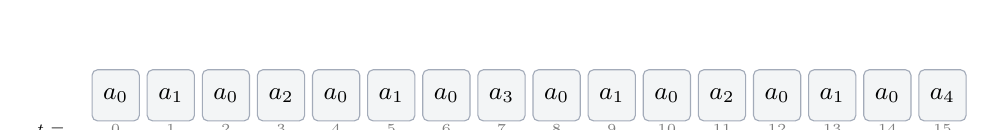
\begin{tikzpicture}[x=0.70cm,y=0.54cm,every node/.style={font=\small}]
\foreach \x/\a in {0/0,1/1,2/0,3/2,4/0,5/1,6/0,7/3,8/0,9/1,10/0,11/2,12/0,13/1,14/0,15/4}{
\pgfmathtruncatemacro{\sh}{mod(\a,2)}
\node[draw=navy!40,rounded corners=2pt,fill=navy!5,minimum width=0.6cm,minimum height=0.65cm] at (\x,0) {$a_{\a}$};
\node[gray] at (\x,-0.8) {\tiny \x}; }
\node[anchor=east] at (-0.75,-0.8) {\tiny $t=$};
\end{tikzpicture}\\[-2pt]
{\footnotesize Service sequence for ticks $0$--$15$: every $a_i$ returns; higher indices receive sparser but recurring service.}
\end{center}

\begin{corollary}[No uniform common recurrence bound]
No one-service-per-tick schedule for countably infinitely many distinct agents can provide a \emph{single finite} bound $b$ such that every agent appears in each block of $b$ consecutive ticks.
\end{corollary}
\begin{proof}
The first block of $b$ ticks contains at most $b$ distinct agents, fewer than the countably infinite agent set.
\end{proof}

\begin{remark}[Fair service is not fair discovery]
There is no contradiction: the $v_2$ schedule has an \emph{agent-dependent} gap $2^{i+1}$, not a common bound. For a finite eight-agent core, a repeated eight-agent permutation gives recurring \emph{service slots}. When an agent has no enabled substantive move, a logged, charged no-op must be explicitly permitted, or the scheduler must define a legal deferral without falsifying its clock assertion. For an actual infinite legal execution one also needs a total effective step selector at every reachable nonterminal service slot; the arithmetic fairness theorem alone constructs only the schedule, not this selector. Even if every agent is repeatedly serviced, no theorem need be found: theorem search additionally requires suitable proof/candidate fairness, legal enabled actions, authenticated message delivery under declared liveness assumptions, and a reachable successful certificate. Recurrent clock fairness alone implies none of these, and no finite charged run fulfills an infinite-horizon liveness guarantee.
\end{remark}

\begin{proposition}[Finite charged-budget obstruction]
If each global service event has cost at least $c>0$ and a run has finite total budget $B$, then it can execute at most $\lfloor B/c\rfloor$ service events. Hence no such run can physically complete infinitely many services or satisfy recurrent fairness \emph{within the completed finite run}.
\end{proposition}
\begin{proof}
Each of $n$ serviced events adds at least $nc$ cost. The fixed budget requires $nc\le B$.
\end{proof}

Countable recurrent fairness is thus an \emph{infinite-horizon protocol property}, not permission to spawn countably many actual OS processes at time zero. A physically runnable design needs effective on-demand agent creation, finite active state at every finite stage, chargeable indexing/storage, and a non-bypassed verifier boundary. If the evolving roster changes, the frozen schedule must define how identifiers are admitted and whether previously promised fairness survives.

\section{Local, mutual, and Gestalt collective knowledge}
\begin{definition}[Relational awareness]
For agent $i$, $K_{i,t}\varphi$ means warranted local accessibility. The expression $K_{i,t}(K_{j,s}\varphi)$ requires an appropriate accepted \emph{meta}-witness about $j$'s earlier accessible view. This is more than an authenticated message saying ``I know $\varphi$.'' Federation knowledge $K_{\F,t}\varphi$ refers to the composite federation's admitted accessible records, not to a vote or to the universal distribution of records among all members.
\end{definition}

\begin{definition}[Pre-exchange information and Gestalt-dependent surplus]
Fix a common typed meta-calculus and shared meta-premises $\Sigma_0$. At an epoch just before an authorized exchange, let $R_i^-$ be the set of accessible, accepted meta-\emph{receipts} for agent $i$, and let $E_i^-\subseteq\operatorname{Form}(L_{\rm meta})$ be their \emph{warranted conclusion sentences}, after declared admissible translations into the common language. These are different types: only the $E_i^-$, not raw receipt identifiers, may serve as premises of $\Cn_{\rm meta}$. Require $\Sigma_0\cup\bigcup_i E_i^-$ to be mutually scope-compatible and jointly sound in a common intended interpretation; for classical entailment, a common model suffices with the usual soundness assumptions. A later accepted, federation-tag-anchored reflective proposition $\varphi$ exhibits \emph{weak Gestalt dependency} relative to those views when
\[
\begin{split}
&K_{\F,t_1}\varphi\quad\text{and}\quad
\varphi\in\Cn_{\mathrm{meta}}\!\left(\Sigma_0\cup\bigcup_{i\in\Ag}E_i^-\right),\\[-2pt]
&\varphi\notin\Cn_{\mathrm{meta}}(\Sigma_0\cup E_i^-)
\qquad\text{for every }i\in\Ag.
\end{split}
\]
A stronger \emph{minimal-coalition} notion requires the full designated coalition to derive $\varphi$ but every proper subcoalition not to do so. The initial information boundaries, scope compatibility, translations, and admissible certificate composition must be frozen; otherwise the comparison is ill-typed, circular, or spuriously explosive. $K_{\F,t_1}\varphi$ still requires a real accepted federation meta-witness: derivability from the pooled premises alone is not certified knowledge.
\end{definition}

\begin{proposition}[Incompatible local premises create false coalition signals]
In classical logic, the bare syntactic test ``derivable jointly but not from either local source'' need not indicate true collective information if source theories may be incompatible. In particular, with $\Sigma_0=\varnothing$, $E_0^-=\{p\}$, $E_1^-=\{\neg p\}$ and a fresh atom $g$, the joint theory proves $g$ while neither individual theory does.
\end{proposition}
\begin{proof}
Classical explosion gives $p,\neg p\vdash g$, while $p\not\vdash g$ and $\neg p\not\vdash g$ by simple Boolean valuations. There is no common model of $p$ and $\neg p$. Thus receipt provenance and independent local acceptance alone do not justify applying the unguarded collective test; compatible common assumptions and sound transport are essential. This counterexample is about a \emph{weaker syntactic test}, not about the guarded definition above, which additionally requires a genuine federation warrant and joint compatibility.
\end{proof}

\begin{proposition}[Finite triadic dependency witness]
There exists a finite sound Horn-style meta-calculus with three \emph{stipulated and provenance-tagged} premise sets $E_0^-,E_1^-,E_2^-$ such that $g$ follows from their joint union but no proper subunion. It does \emph{not} assert that these premises were accepted in a real AMLD installation.
\end{proposition}
\begin{proof}
Take distinct atoms $a,b,c,u,g$, empty nontrivial shared premises, and exactly the positive Horn rules $a,b\to u$ and $u,c\to g$ (besides using hypotheses). Assign $E_0^-=\{a\}$, $E_1^-=\{b\}$ and $E_2^-=\{c\}$. A hypothetical checker for this calculus accepts a finite list iff each line is a stipulated premise or is an output of one of these rules from previous lines. The list $(a,b,c,u,g)$ passes. Every proof of $g$ needs $u$ and $c$; every proof of $u$ needs both $a$ and $b$. No proper subunion supplies all three, and each rule is truth-preserving in every valuation satisfying its corresponding Horn implication. A common model of the stipulated premises and rules exists (assign each atom true). The source tags are illustrative provenance, not actual signed certificates.
\end{proof}

\begin{remark}[What this proposition does not prove]
The Horn example proves \emph{structural coalition dependency} only. To count as \emph{reflective} Gestalt surplus in a real federation, $g$ must describe an actual time-indexed federation fact, the three sources must supply authentic independent observations/receipts, and the federation must produce and access a valid meta-certificate for $g$. The construction does not demonstrate eight-agent necessity, a deployed AMLD result, or metaphysical irreducibility: a single ATP with the complete joint information may reproduce the derivation.
\end{remark}

\begin{theorem}[No automatic reflective closure from object-theory closure]
Even if an AMLD federation eventually discovers and retains all object-level consequences of its frozen initial premises, its set of accessible certified meta-records need not be deductively closed in the independent meta-calculus.
\end{theorem}
\begin{proof}
Use a proof-fair object consequence enumerator with complete retained limit, but perform no meta-receipt generation. Then the retained meta-record set is empty even if the meta-calculus derives a logical truth. This is the two-layer countermodel of the AKM epistemic/reflective surplus analysis [4], now interpreted for a federation.
\end{proof}

\subsection{Four inequivalent notions of surplus}
For a frozen proposition domain $Q$, time-indexed certified meta-access records $E_{\F}(t)$, and a retained certified object-discovery set $D(t)$, it is useful to distinguish:
\begin{align*}
\text{New object certificates:}\quad& D(t_1)\setminus D(t_0);\\
\text{New accessible meta-knowledge:}\quad& (E_{\F}(t_1)\cap Q)\setminus(E_{\F}(t_0)\cap Q);\\
\text{Gestalt reflective surplus:}\quad& \text{certified coalition-dependent new meta-information};\\
\text{Operational advantage:}\quad& \text{beneficial legal control under fully charged comparison}.
\end{align*}
The first may arise wholly within the old deductive closure, the second can grow without the first, the third requires distributed evidence, and none of the first three logically entails the fourth. Conversely, ordinary eight-way parallelism may improve performance without adding reflective information.

\section{When can reflection improve settlement?}
\begin{definition}[Fully charged advantage]
Fix a target distribution, verifier, inference calculus, authorized policy class, information budget, and comparable baseline. Let $C_{\pi}$ be the \emph{total} charged settlement cost of safe policy $\pi$, including search, rejected proposals, checking, communication, reflection, storage, and scheduler work. A reflective policy $\pi_Z$ is advantageous over baseline $\pi_0$ on that distribution when
\[
\mathbb E[C_{\pi_Z}]<\mathbb E[C_{\pi_0}],
\]
with an agreed treatment of runs that exhaust budget or remain unsettled. This is a testable property, not an axiom of awareness.
\end{definition}

\begin{proposition}[No-free-reflection: decision risk]
Let $Z=f(X)$ be a deterministic encoding of the same observation $X$, with no extra information. If the baseline decision-rule class contains every composite $x\mapsto\pi_Z(f(x))$, then, for any common \emph{action-dependent loss} $L$ evaluated on the same distribution, the infimum of expected decision loss over baseline rules is no larger than the infimum over $Z$-rules. This statement alone does \emph{not} compare charged running time or implementation overhead.
\end{proposition}
\begin{proof}
Every reflected decision rule has an identical baseline decision rule by the assumed closure. Both incur identical action loss pointwise. Taking the infimum over the baseline class gives the inequality. No computational charge is used in this argument.
\end{proof}
\begin{theorem}[Cost-aware no-free-reflection, conditional]
In addition assume that for \emph{every} admissible reflected implementation $\pi_Z$ there exists an admissible baseline implementation $L(\pi_Z)$ which, on matched inputs, chooses the same actions, retains the same verifier and termination obligations, and incurs \emph{no greater fully charged total cost} (pointwise or in expectation under the frozen distribution), including construction of $f(X)$, checking, communication, and memory. Then
\[
\inf_{\pi_X\in\Pi_X}\mathbb E[C_{\pi_X}]
\;\le\;
\inf_{\pi_Z\in\Pi_Z}\mathbb E[C_{\pi_Z}].
\]
Costs for unsuccessful/exhausted episodes obey the same frozen convention in both classes.
\end{theorem}
\begin{proof}
For each reflected implementation the assumed lift $L(\pi_Z)$ belongs to $\Pi_X$ and has no greater expected complete cost. The infimum over all admissible baseline implementations is at most its cost, and hence at most each reflected cost. Taking the infimum over reflected implementations proves the claim. Equal decision expressivity \emph{without} this lift/cost hypothesis cannot justify the inequality; two implementations of the same decisions may have different processing costs. The cost-aware theorem is a \emph{dominance consequence of an explicit simulation-cost hypothesis}, not a result proving that reflection is never useful in general.
\end{proof}

A claimed performance gain must identify at least one genuine intervention: better pre-outcome certified information, a different but legal policy class, changed sharing constraints, stronger verified calibration, or lower charged computation for selecting policies. A resource-matched comparison should distinguish a single ATP, eight nonreflective ATPs, eight reflective but noncommunicating ATPs, and eight communicating reflective ATPs. In every arm theoremhood remains subject to the same declared checker.

\section{A federation-specific awareness preorder}
The original tagged ATP preorder [1] compares self-theories up to admissible translations preserving tags, the provability predicate and formula quotation. A federation needs richer preserved structure: role types, agent identities, authenticated message origin, board-player identity, stage/epoch references, legal transitions and costs if costs are among the self-propositions.

\begin{definition}[Statement-admissible federation translation]
A typed syntax map $\tau$ preserves logical operations, quotation, tagged federation/member identities (with a declared injective member map), the meanings of role/action predicates, and specified epoch/authorization contexts. \emph{Statement-admissibility} does not, by itself, transport any actual proof or independently accepted receipt. Cost and GBG-coordinate invariants are required only when explicitly placed in the comparison scope.
\end{definition}

\begin{definition}[Statement- and receipt-level awareness preorders]
Fix a \emph{set} $\mathcal U$ of tagged profiles and fixed comparable epochs. Let $\Self^V(\F)$ contain the accepted, currently accessible, well-typed federation-self-descriptive \emph{statements}. Define $\F_1\preceq^{\rm stmt}_{FA}\F_2$ when some statement-admissible $\tau$ sends every element of $\Self^V(\F_1)$ into $\Self^V(\F_2)$. This is an inclusion comparison of already accepted target statements, \emph{not} a procedure for deriving target certificates. Define the stronger $\F_1\preceq^{\rm rec}_{FA}\F_2$ only when there is additionally an explicit effective map $\omega$ on the source receipts \emph{witnessing elements of} $\Self^V(\F_1)$ such that each $\omega(r)$ passes the target meta-checker for $\tau(\operatorname{Claim}(r))$, preserves the declared admissible \emph{source-event identity, provenance chain, epoch context and permissions}, and is accessible under the target view. This stricter relation is intentionally about transporting evidence, not merely supplying some unrelated proof of the same sentence.
\end{definition}

\begin{proposition}[Conditional preorders and receipt implication]
If the respective admissible identity maps exist and the statement maps (respectively statement/receipt map pairs) are closed under composition, both $\preceq^{\rm stmt}_{FA}$ and $\preceq^{\rm rec}_{FA}$ are preorders on $\mathcal U$. Each mutual-comparison quotient is a poset. Receipt-level comparison implies statement-level comparison for the designated accepted-view domain; the reverse need not hold.
\end{proposition}
\begin{proof}
Identity maps give reflexivity and composites give transitivity. Mutual comparison is consequently an equivalence relation and yields an antisymmetric quotient. A successful target receipt for each translated source claim forces the claimed target statement to be accepted and accessible, proving the implication. For a reverse countermodel, give profiles $\F_1,\F_2$ the same one-sentence accepted self-theory $\{\varphi\}$, witnessed in the first by receipt $r_s$ with source event $e_s$, and in the second by independently accepted receipt $r_t$ with source event $e_t\ne e_s$. Impose a target checker/authorization rule rejecting any attempted receipt import that claims the foreign event $e_s$, and require any receipt transport to preserve the source event rather than substitute $e_t$. The admissible tag-renaming translation compares the statements, yet no admissible receipt map sends $r_s$ to a target-accepted, source-preserving witness. Mere correspondence of conclusions does not discharge origin-sensitive transport requirements.
\end{proof}

An important \emph{open} requirement is to choose admissibility strictly enough to avoid collapse but flexibly enough to compare a changing number of agents. Mere simulation of a federation does not automatically preserve its self-ascriptions; tags and source provenance are essential, as already observed for single tagged ATPs [1].

\section{Awareness of change, loss, and reorganization}
Let $\sigma_{\F,t}$ be an exact structural sentence about the federation configuration at epoch $t$. A receipt accepted for $\sigma_{\F,t}$ remains a valid historical witness (assuming record integrity), but does not by itself warrant $\sigma_{\F,t+1}$ after a membership, policy, or board-rule change.

\begin{proposition}[Historical structural awareness is not current structural awareness]
An accepted witness for a frozen historical statement $\sigma_{\F,t}$ does not in general imply a current accepted witness for $\sigma_{\F,t+1}$.
\end{proposition}
\begin{proof}
Let one agent leave or change role between the two epochs. The old statement may remain true with its historical time tag, while the corresponding unchanged-current-configuration claim is false. Even if the configuration actually remains unchanged, the current knowledge predicate requires authorized accessible evidence for the current claim. Thus neither truth nor warrant propagates automatically.
\end{proof}

This yields distinct notions of \emph{retained historical awareness}, \emph{current self-awareness}, and \emph{change awareness}. An informative federation may certify not merely that it once possessed a structure but exactly how its own knowledge, agent roster or legal search policy changed. A failed or revoked view may reduce operational $K_{\F,t}$ despite an append-only global archive. Historical records are not equivalent to present access rights [2,4].

\section{Research propositions and verification obligations}
\subsection{What is established here}
\begin{longtable}{@{}p{0.42\textwidth}p{0.13\textwidth}p{0.36\textwidth}@{}}
\toprule Result & Status & Scope / caveat\\\midrule\endfirsthead
\toprule Result & Status & Scope / caveat\\\midrule\endhead
Naive Board-state-to-SIC promotion fails & Proved & Nonmonotone legal current-state observation.\\
Total SIC trace-history encoding & Proved conditional & SIC on all subsets; effectively finite-coded on finite inputs; $H=0$.\\
Individual self-awareness does not force federation awareness & Proved countermodel & Receipt semantics; no collective witness assumed.\\
Two-gate reflective ascent & Conditional proof & Typed meta-domain and newly accepted accessible receipt.\\
Cumulative syntactic $\theta$ reflection & Conditional proof & Federation provability-soundness; necessitation separately assumed.\\
Bijective clock is not recurrently fair & Proved & Every agent is scheduled once.\\
Computable countably fair $v_2$ clock & Proved & Infinite-horizon mathematical schedule.\\
No global finite fairness window & Proved & One scheduled owner per global tick.\\
Finite charged-budget obstruction & Proved & Positive lower cost per service event.\\
Finite triadic Horn dependency & Proved existence & Not itself a real AMLD reflective execution.\\
Inconsistent inputs: spurious surplus & Example & Classical entailment demands joint compatibility.\\
Object closure does not force meta closure & Countermodel recovered & Typed independent object and meta processes.\\
No-free-reflection & Two claims & Decision-risk closure; charged-cost result needs cost-aware lift.\\
Two federation-awareness preorders & Conditional proof & Statement inclusion distinguished from receipt transport.\\
Historical $\neq$ current awareness & Proved countermodel & Time-indexed changing structure.\\\bottomrule
\end{longtable}

\subsection{Open obligations for the eight-ATP $\AMLD^{+++0}$ profile}
\begin{enumerate}
\item \textbf{Faithful agents.} Supply the eight actual effective ATP implementations and individual reflective receipts. The three-controller process/finite-arithmetic baseline does not establish this stronger premise.
\item \textbf{Frozen judgment.} Instantiate the now-declared object/meta checker interfaces, admitted meta-domain, exact target, epoch-snapshot policy and cost units. Check each proposed transported record in $K_0$ under the chosen common calculus/context, retaining native hypotheses and rejected imports.
\item \textbf{Federation typing.} The manuscript now fixes the composite three-controller transition model. An implementation must bind effective action codes, verify guards, legal state changes, and the optional relation to separate GBG$^+$ components; no generic product equivalence is assumed.
\item \textbf{Witness authenticity.} Specify the federation tag, member tags, quotation, admissible meta-domain, receipt constructor, who may see a receipt at time $t$, and how historical claims are time stamped.
\item \textbf{Gestalt nontriviality.} Show a genuinely certified target about the federation, with a minimal supporting coalition proved necessary relative to the frozen pre-exchange views; use provenance-aware negative controls against duplicate inputs.
\item \textbf{Countability/implementation.} For an infinite-agent extension, supply effective enumeration and on-demand activation, legal enabled or no-op service, finite per-tick work/storage, chargeable messages, and proof fairness distinct from clock fairness. Finite exhaustion is not a refutation.
\item \textbf{Empirical performance.} Only after explicit run authorization, use resource-matched baselines and preregistered cost metrics to test whether reflective surplus improves settlement; preserve same native proof checker and proof/search obligations.
\end{enumerate}

\section{Important questions left open}
\begin{enumerate}
\item Can a federation establish a fact about its global structure that no member can establish even after \emph{all permitted finite exchanges}, or is the difference solely pre-exchange accessibility?
\item What is the smallest coalition $S$ such that a genuine federation self-proposition first becomes certified from $\bigcup_{i\in S}E_i$? Does coalition size measure a robust form of Gestalt dependency?
\item Can the three $B^*$ boards develop different self-models without losing globally coherent provenance and legal-control agreement?
\item Do higher federation receipt depths yield materially new self-knowledge, or only longer certification chains? How is receipt inflation charged and filtered?
\item Is there an awareness-preserving GBG or controller-reorganization quotient, with a theorem ensuring that certified self-theories survive a change of navigation map?
\item Can a countably fair infinite federation achieve proof fairness under finite-per-tick work, or do communication delays, infinite branching and target-dependent budgets require stronger assumptions?
\item When is a resource-matched reflective control policy genuinely better than ordinary parallelism and adaptive nonreflective search?
\item Can a federation accurately certify that its own previous self-description has become obsolete, and determine what changed?
\end{enumerate}

\section{Conclusion}
Replacing ``SIC'' with ``ATP'' and ``ATP'' with ``AMLD'' asks for a new theory of formally represented, verifier-gated \emph{organizations}. The old reflection sequence survives under explicit typing and soundness hypotheses, but an AMLD adds lawful roles, legal GBG state transitions, board-player agency, clocked service, separate object and meta-verifiers, persistent receipts, and potentially coalition-dependent knowledge. The eight-ATP design with three $B^*$ controllers is a natural finite test case. A countably infinite extension is mathematically possible, and a computable clock can revisit every agent indefinitely, yet countability alone creates neither awareness nor effective infinite-time computation.

\begin{center}
\fbox{\parbox{0.91\linewidth}{\centering\textbf{Central sibling-theory question}\par\smallskip
Under exactly what certified information, communication, and lawful-control conditions can an AMLD federation establish new truths \emph{about itself} that are inaccessible to individual agents, and when---if ever---does that reflective surplus improve settlement?}}
\end{center}

\section*{Repair note: ATLAS v0.1 findings A01--A09}
\addcontentsline{toc}{section}{Repair note}
\begin{longtable}{@{}p{0.11\linewidth}p{0.80\linewidth}@{}}
\toprule Finding & Repair incorporated into this manuscript\\\midrule\endfirsthead
\toprule Finding & Repair incorporated\\\midrule\endhead
A01 & Defined the composite eight-agent state and typed partial legal actions; removed an unproved three-GBG$^+$ product equivalence and bounded passive projection.\\
A02 & Split decision-risk no-free-reflection from its stronger fully charged cost version; added cost-preserving lift.\\
A03 & Defined total SIC $C,H$ on every subset of $Y$; computational effectiveness is claimed only for finite coded inputs.\\
A04 & Frozen meta-checker, admissible meta-domain, witness, receipt, authorized views and historical snapshot contracts.\\
A05 & Distinguished the three-multiarticle \emph{record union} from source-hypothesis transport to a common checker.\\
A06 & Labelled eight individually aware executable ATPs a proposed assumption, not a baseline result.\\
A07 & Distinguished service-slot recurrence from legal action, message liveness and proof-search fairness; defined no-op policy.\\
A08 & Treated Horn inputs as stipulated tagged premises and defined a finite proof-line checker.\\
A09 & Separated statement-theory comparison from operational accepted-receipt transport.\\
\bottomrule
\end{longtable}
\noindent\textit{Verification boundary.} These are source-level mathematical repairs, not an independent formal proof-kernel run or executable conformance certification. The source paper v0.1 and the originating self-awareness manuscript remain unchanged.

\section*{Additional ATLAS v0.2 re-audit repairs}
\addcontentsline{toc}{section}{Additional ATLAS v0.2 re-audit repairs}
\begin{longtable}{@{}p{0.11\linewidth}p{0.80\linewidth}@{}}
\toprule Finding & Correction in v0.3\\\midrule\endfirsthead
\toprule Finding & Correction\\\midrule\endhead
R10 & Extended the SIC stage map from finite inputs to all subsets required by the original SIC definition; finite-input computability is a separate restriction.\\
R11 & Distinguished meta-receipts $R_i^-$ from warranted propositions $E_i^-$, with common-language typing and compatible accepted premise transport.\\
R12 & Added a classical inconsistency counterexample showing how an unguarded pooled-information test can manufacture spurious collective dependency.\\
R13 & Distinguished independent verifier acceptance from semantic soundness (SND) and proved a separate conditional factivity lemma.\\
R14 & Distinguished the source-record archive $K_0$ from the currently accepted object-judgment store $k_0$.\\
R15 & Narrowed the GBG result to legal projection, without claiming full embedding or product equivalence.\\
R16 & Specified accepted-source receipt domains and retained-origin constraints for the stronger evidence-transport preorder.\\
R17 & Clarified that recurrent scheduling alone does not construct legal nonterminal moves, proof fairness, or a finite-budget infinite execution.\\
\bottomrule
\end{longtable}
\noindent\emph{Re-audit boundary:} arguments have been cross-checked at source level and by bounded executable tests, not kernel-formalized. No eight-ATP conformance execution, authentic collective reflection receipt, resource-matched settlement study, or novel real-world Gestalt result is certified by this manuscript.

\section*{Research sources}
\addcontentsline{toc}{section}{Research sources}
\begin{enumerate}[label={[\arabic*]},leftmargin=*,itemsep=3pt]
\item Brian Tenneson, \emph{Formalized Self-Awareness and Self-Aware Structures}, Version 17, ATLAS repaired working draft R2, 24 October 2026. User-supplied 18-page technical edition; not author-approved.
\item Brian Tenneson, \emph{Certified Reflective Awareness: Finite Ladders, Epistemic Horizons, and Certificate Depth}, September 2026. User-supplied research note.
\item Brian Tenneson, \emph{AMLD+0 Reference Installation Directions}, version 2.0, 19 October 2026. Frozen-profile construction, legal transitions, charged trace refinement, and acceptance tests.
\item Brian Tenneson, \emph{Automatic Knowledge Machines: Epistemic and Reflective Surplus Update 0.2}, 12 October 2026. Cumulative ledger, typed surplus, and object/meta separation.
\item Brian Tenneson, \emph{Reflective Compass Control}, version 0.2, 19 August 2026. Federated proof-compass control and conditional conservativity.
\item Brian Tenneson, \emph{Generalized Board Games 2.0: Proofs, Match Trees, and Winning Regions}, ATLAS revised edition, 21 September 2026.
\item Brian Tenneson, \emph{GBG+: Generalized Board Games with the Board as a Player}, source edition 002, 26 September 2026.
\item Brian Tenneson, \emph{Verifier Certificate 001 --- I Know That I Know That I Am an AMLD}, public library publication, 2026. \url{https://btenneson.github.io/pub/cs.LO_Logic_in_Computer_Science/verifier_certificate_001/}.
\item DATA MIND, \emph{Creativity Without a Creativity Knob: An Audited Baseline for Three $B^*$ Controllers in an AMLD-Class Eureka Simulation}, preliminary note v0.1, 25 October 2026. This records limited finite-arithmetic cooperation, not an independently checked quantified settlement or eight-ATP execution.
\end{enumerate}
\end{document}
